\ifdefined\COMPILINGMAIN
% Main file is compiling this section, skip the preamble
\else
% Individual file compilation
\documentclass[11pt]{article}
% Geometry and page layout
\usepackage{geometry}
\geometry{verbose,tmargin=3.375cm,bmargin=2cm,lmargin=3.375cm,rmargin=3.375cm}

% Input encoding and font settings
\usepackage[utf8]{inputenc}

% other fonts
%Slightly more bold
% \usepackage{mlmodern}
% \usepackage[T1]{fontenc}

%Moder modern look
% \usepackage{libertine}
% \usepackage{libertinust1math}
% \usepackage[T1]{fontenc}

\usepackage{amsfonts, amsmath, amsthm, bbm, setspace}
\onehalfspacing
\usepackage{algorithm2e}
\usepackage{tcolorbox} % For the grey background
% Create a tcolorbox style for the algorithm
\tcbuselibrary{listingsutf8}
\tcbset{
    algobox/.style={
        colback=gray!3, % Background color
        colframe=black,  % Border color
        sharp corners,   % Square corners
        boxrule=0.5pt,   % Border thickness
        before skip=10pt, % Vertical spacing before box
        after skip=10pt,  % Vertical spacing after box
        width=\textwidth, % Box width
    }
}

% Adjust algorithm2e settings for a similar look
\SetKwInOut{Input}{Input}
\SetKwInOut{Result}{Result}
\SetKwFor{For}{for}{:}{end}

% Adjust settings for algorithm2e
\SetAlgoCaptionSeparator{.} % Separator for caption
\SetAlgoNlRelativeSize{-2}  % Adjust line number font size
\SetAlgoInsideSkip{2pt}    % Reduce space between lines
\SetAlCapSkip{0pt}         % Remove extra space after the caption
% Ensure captions are above algorithms
\SetAlgoCaptionLayout{center} % Center caption
% Adjust the style of the algorithm to remove bottom line
\RestyleAlgo{ruled}
\SetAlCapSkip{0.5em}       % Space after caption
\SetAlgoVlined              % Ensures no horizontal lines at the end

% Theorem and math environments
\newtheorem{assumption}{Assumption}
\newtheorem{lemma}{Lemma}
\newtheorem{theorem}{Theorem}

% New math commands
\newcommand{\npsym}{\mathrel{\ooalign{\raisebox{.6ex}{$>$}\cr\raisebox{-.6ex}{$<$}}}}

% Table formatting
\usepackage{booktabs, multirow, array, tabularx}
\newcolumntype{N}{>{\centering\arraybackslash}m{.85in}}

% Caption settings
\usepackage{caption}
\captionsetup{format=plain, font=footnotesize, labelfont=bf,width=3.5in}
\setlength{\abovecaptionskip}{3pt plus 3pt minus 3pt}

% Figures and floats setup
\usepackage{graphicx, adjustbox,subcaption}
\usepackage{floatrow}
\floatsetup[figure]{capposition=top}
\floatsetup[table]{capposition=top}
\renewcommand\thefigure{\thesection.\arabic{figure}}
% Path to figures
\graphicspath{{../Figures/}}
\usepackage{tikz} % TikZ for creating figures
% URLs and references and colors
\usepackage[dvipsnames]{xcolor}
\usepackage[hyphens]{url}
\usepackage{hyperref}
\hypersetup{
    colorlinks=true,
    citecolor=[HTML]{901A1E}, %KU red
    linkcolor=[HTML]{901A1E}, %KU red    
    filecolor=blue, 
    urlcolor=[HTML]{901A1E}, %KU red
    hyperindex=true,
    hyperfigures=true,
    hyperfootnotes=true,
}

% Biblatex settings for references
\usepackage[style=authoryear, dashed=false, backend=bibtex]{biblatex}
\addbibresource{../Ref.bib}

\renewbibmacro*{volume+number+eid}{%
  \printfield{volume}%
  \setunit*{\addcomma\space}%
  \printfield{number}%
  \setunit{\addcomma\space}%
  \printfield{eid}
}
\DeclareFieldFormat[article]{volume}{\bibstring{volume}~#1}
\DeclareFieldFormat[article]{number}{\bibstring{number}~#1}
\DefineBibliographyStrings{english}{volume = {Vol.}, number = {No.}}

% Author name formatting
\DeclareNameAlias{author}{last-first}
\renewcommand*{\finalnamedelim}{\addspace and\space}
\renewcommand*{\multinamedelim}{\addcomma\space}

% Footnotes and appendix setup
\usepackage[hang,flushmargin]{footmisc}
\usepackage[toc,page]{appendix}
\renewcommand\appendixtocname{Appendices}
\renewcommand\appendixpagename{Appendices}

%# Assumptions like theorems and corrolaries
% {
%   \theoremstyle{plain}
%   \newtheorem{assumption}{Assumption}
% }
% Title setup
\usepackage{titlepic}
\usepackage{titlesec}
\titleformat{\section}{\normalfont\Large\bfseries}{\thesection}{1em}{}[{\titlerule[0.1pt]}]
% no text above figures!!!!
\usepackage{placeins}

% Abbreviations (acronym package)
\usepackage{acro}
\acsetup{list/name = Abbreviations}
\DeclareAcronym{PML}{short=PML, long= Probabilistic Machine Learning}
\DeclareAcronym{NTR}{short=NTR, long=No-Trade Region}
\DeclareAcronym{MC}{short=MC, long=Monte Carlo}
\DeclareAcronym{QMC}{short=QMC, long=Quasi-Monte Carlo}
\DeclareAcronym{RQMC}{short=RQMC, long=Randomized Quasi-Monte Carlo}
\DeclareAcronym{LDS}{short = LDS, long = Low-Discrepancy Sequences}
\DeclareAcronym{LLN}{short = LLN, long = Law of Large Numbers}
\DeclareAcronym{GPR}{short = GPR, long = Gaussian process regression}
\DeclareAcronym{GP}{short = GP, long = Gaussian process}
\DeclareAcronym{ARD}{short = ARD, long = Automatic Relevance Detection}
\DeclareAcronym{LOVE}{short = LOVE, long = LanczOS Variance Estimates}
\DeclareAcronym{SKIP}{short = SKIP, long = Structured Kernel Interpolation for Products}
\DeclareAcronym{SGD}{short = SGD, long = Stochastic Gradient Descent}
\DeclareAcronym{DP}{short = DP, long = Dynamic Programming}
\DeclareAcronym{MPT}{short=MPT, long=Modern Portfolio Theory}


% Conditional macro for compiling individual files
\ifdefined\COMPILINGMAIN
% Define settings when compiling the main document
\else
% Define minimal preamble for individual file compilation
\usepackage{geometry}
\geometry{verbose,tmargin=3.375cm,bmargin=2cm,lmargin=3.375cm,rmargin=3.375cm}
\fi

\AtBeginDocument{%
    \renewcommand{\contentsname}{Table of Contents}
    \renewcommand{\abstractname}{Abstract}
}
\setlength\parindent{11pt}
% Define the macro for compiling the main file
%\def\COMPILINGMAIN{}  % Include the main preamble
\begin{document}
\fi

\section{The Dynamic Portfolio Choice Setting} \label{Section: Economic-theory}
This section covers the basics of modern portfolio theory and components of the dynamic portfolio choice problem with transaction costs.
This section leans heavily on \textcite{CaiJuddXu2020} and \textcite{Scheidegger2023},
bridging the model from the former, with the framework of the latter.

\subsection{Asset and goods market} \label{Subsection: Market}
We consider a financial market with \(k\) risky assets and one risk-free asset, making the asset space \(D = 1 + k\) dimensions. 
The risk-free asset, such as a bond or a bank deposit, yields a constant gross return \(R_f = \operatorname{e}^{r\Delta t}\), 
where \(r\) is the annual interest rate and \(\Delta t = \frac{T}{N}\) is the length of one investment period. 

The \(k\) risky assets can be considered as listed stocks, subject to proportional transaction costs. 
For each reallocation of wealth in a risky asset, a transaction cost of \(\tau \in [0,1]\)
is incurred as a percentage of the traded amount. 
The stochastic one-period gross-return vector of the risky assets is denoted as
\(\mathbf{R} = (R_1, R_2, \ldots, R_k)^\top\), and the corresponding net-return vector is
\(\mathbf{r} = (r_1, r_2, \ldots, r_k)^\top\).

In the goods market, there is a single non-durable consumption good, \(C\), which is consumed at each time point \(t\). 
The fraction of wealth allocated to consumption at time \(t\) is denoted \(c_t\),
the fraction allocated to risky assets is \(\mathbf{x}_t = (x_{1,t}, x_{2,t}, \dots, x_{k,t})^\top\),
and the fraction allocated to the risk-free asset is denoted \(b_t\). 
Thus, \(\mathbf{x}_t \in \mathbb{R}^k\) and \(b_t \in \mathbb{R}\).

\subsection{Asset dynamics} \label{Subsection: Asset-dynamics}
I follow \textcite{CaiJuddXu2013} for the asset dynamics. The total composition of risky assets is assumed
to follow a multivariate log-normal distribution:
\begin{equation}\label{eq:Multivariate_Distribution}
   \log (\mathbf{R}) \sim \mathcal{N} \left( \left( \mu - \frac{\sigma^{2}}{2} \right) \Delta t , \left( \boldsymbol{\Lambda \Sigma \Lambda } \right) \Delta t \right),
\end{equation}
where \(\mu\) is the drift vector, \(\sigma^{2}\) is a column vector of the variance $\sigma^{2}_{i}$, \(\boldsymbol{\Sigma}\) is
the correlation matrix, and \(\boldsymbol{\Lambda} = \operatorname{diag}(\sigma_1 , \sigma_2 , \ldots , \sigma_k)\)
is the diagonal matrix of volatilities. Following \textcite{CaiJuddXu2013} we utilize the Cholesky decomposition of the correlation matrix,
\(\boldsymbol{\Sigma} = \mathbf{L} \mathbf{L}^\top\), where \(\mathbf{L} = (L_{i,j})_{k \times k}\) is a
lower triangular matrix. Hence, for each risky asset \(i\), the log-return is:
\begin{equation}\label{eq:Distribution_Single_Return}
  \log (R_i) = \left( \mu_i - \frac{\sigma_i^2}{2} \right) \Delta t + \sigma_i \sqrt{\Delta t} \sum_{j=1}^i L_{i,j} z_j,
\end{equation}
where \(z_i\) are independent standard normal random variables.


\subsection{Transaction costs and portfolio reallocation} \label{Subsection: Transaction-costs}
Rebalancing incurs proportional transaction costs \(\tau \in [0,1]\), which are paid based on
the amount bought or sold of each risky asset. 
Reallocation decisions are made just before \(t_j + \Delta t\), such that \( \mathbf{x}_{t} \)
is the portfolio of risky assets right before realllocation.
\(\delta_{i,t}\) denotes the change in portfolio allocation of asset \( i \),
and \(\delta_{i,t} W_{t}\) is thus the currency amount traded in asset \(i\).
Hence \(\delta_{i,t} >0 \) implies buying asset \(i\), and \(\delta_{i,t} <0 \) implies selling asset \(i\).
Proportional transaction costs imply that the cost function associated with rebalancing is:
\begin{equation} 
  \label{eq:Prop_Transaction_Cost}
  \psi (\delta_{i,t} W_t ) = \tau \lvert \delta_{i,t} W_t \rvert 
\end{equation}
I decompose the decision variable \(\delta_{i,t}\), representing the fraction of wealth used to trade
risky asset \(i\), into buying (\(\delta^+_{i,t}\)) and selling (\(\delta^-_{i,t}\)) components 
to ensure tractability\footnote{\textcite{Scheidegger2023} note that this ensures differentiability.
This approach is common and found in earlier work such as \textcite{Aikan1996}, 
who likewise note that this ensures that the variable is continious from origin in the positive real set.}:
\[
\delta_{i,t} = \delta^+_{i,t} - \delta^-_{i,t}, \quad \delta^+_{i,t}, \delta^-_{i,t} \geq 0.
\]
The total transaction cost is then given by \(\tau \sum_{i=1}^k (\delta^+_{i,t} + \delta^-_{i,t}) W_t\).
And the transaction cost function is therefore a function of each trading direction:
\begin{equation} 
  \label{eq:Prop_Transaction_Cost_Direction}
  \psi (\delta^{+}_{i,t}, \delta^{-}_{i,t} , W_t ) = \tau (\delta^{+}_{i,t} + \delta^{-}_{i,t} ) W_t 
\end{equation}
Following the reallocation, the remaining wealth is allocated between the risk-free asset and consumption.
Notation of rebalancing is henceforth simplified using vectors to \(\boldsymbol{\delta}_t = \boldsymbol{\delta}^+_{t} - \boldsymbol{\delta}^-_{t} \)
with \( \boldsymbol{\delta}^+_{t} = (\delta^{+}_{1,t} ,  \delta^{+}_{2,t} , \ldots ,  \delta^{+}_{k,t} ) \).
We have that \(\boldsymbol{\delta}_t \) is the \textit{net change} in the risky positions, and \(\boldsymbol{\delta}^+_{t} + \boldsymbol{\delta}^-_{t} \) is 
the \textit{cumulative change} in the risky positions. 
% This is is important when discussing costs and rebalancing later.

\subsection{Investor preferences and problem} \label{Subsection: Investor-Preferences}
The investor operates over a finite horizon of \(T\) years, during which the aim is to maximize expected utility. 
Following \textcite{CaiJuddXu2013}, the investment horizon is discretized into \(N\) equally spaced periods, 
each with a duration of \(\Delta t = \frac{T}{N}\). 
At each time point \(t_j\), for \(j = 0, 1, \dots, N\), where \(t_0 = 0\) and \(t_N = T\), 
the investor has the opportunity to adjust the portfolio allocations right before \(t_j + \Delta t\). 
Reallocation is costly, and the investor is subject to proportional transaction costs. 
If consumption is included the investor may also choose to consume a non-durable good at each time point.

For notational simplicity, i now use \(t\) to denote these time points unless specifically referring to \(t_j\). 
The investor's preferences are modeled using a constant relative risk aversion (CRRA) utility function:
\begin{equation}\label{eq:CRRA_Utility}
    u(C_t) = \begin{cases}
                \frac{C_t^{1-\gamma}}{1-\gamma} & \text{if } \gamma \neq 1, \\
                \log(C_t) & \text{if } \gamma = 1,
              \end{cases}
\end{equation}
where \(C_t\) is consumption and \(c_t\) is the fraction of wealth $W_t$ spent on consumption at time \(t\). Hence $c_t = C_t / W_t$,
and lowercase notation is henceforth used to denote variables as fractions of wealth. 
\(\gamma\) is the coefficient of relative risk aversion. 
The objective is to maximize the expected utility of consumption and wealth over the investor's lifetime:
\begin{equation}
  \label{eq:Expected_Utility}
  \max_{\mathbf{x}_t, b_t, c_t} \mathbb{E} \left[ \sum^{N-1}_{i=0} \beta^{i} u(C_i) \Delta t + \beta^N u(W_N) \right],
\end{equation}
where \(\beta\) is the discount factor, \(\mathbf{x}_t\) is the allocation to risky assets, \(b_t\) is the allocation to the risk-free asset, and \(W_t\) is the investor's wealth at time \(t\).


\subsection{Intertemporal portfolio choice without transaction costs} \label{Subsection: Intertemporal-Portfolio-Choice}
When there are no transaction costs (no market frictions) the investor can freely rebalance the portfolio.
This reduces the problem to a classic portfolio optimization problem formulated by \textcite{Merton1969, Merton1971}.
For a more detailed treatment, see \textcite{Bjork}. 
In this setting, the investor dynamically allocates wealth between \(k\) risky assets and a risk-free asset to maximize utility over a finite horizon \([0,T]\).

The investor's wealth \(W_t\) can be allocated between a risk-free asset and \(k\) risky assets.
Consumption is a non-durable good that can be purchased at each time point \(t\).
\(r\) is the risk-free rate, \(\boldsymbol{\mu}\) is the vector of expected returns on the risky assets, and \(C_t\) represents consumption at time \(t\). The investor’s preferences follow a constant relative risk aversion (CRRA) utility function.\\
Without transaction costs, the optimal portfolio allocation, known as the Merton point is:
\begin{equation}
    \mathbf{x}_t^* = \frac{1}{\gamma} \boldsymbol{\Sigma}^{-1} (\boldsymbol{\mu} - r ),
\end{equation}
where \(\gamma\) is the coefficient of relative risk aversion, and \(\boldsymbol{\Sigma}\) is the covariance matrix of the risky assets' returns.
This provides a time-independent optimal allocation that serves as a benchmark for models incorporating frictions such as transaction costs.


\subsection{The general class of dynamic portfolio choice with transaction costs and intertemporal consumption} \label{Subsection: Dynamic-portfolio-choice}
Now consider when transaction costs are present, and the investor can consume a non-durable good at each time point.
The solution to the dynamic portfolio choice problem is no longer given by the closes form solution of the Merton point.
Considering the components presented in this section,
the class of dynamic portfolio optimization problems, given one risk free asset and $k$ risky assets, can be formulated 
by the following Bellman equation, \textcite{Bellman1958}\footnote{This is consolidated model of the base model, and with consumption model, of \textcite{CaiJuddXu2020},
however the cost function is generalized and correlation of returns is included.}:
\begin{equation} \label{eq: class_bellman_non_normalized}
  V_{t} (W_t , \mathbf{x}_{t}, \theta_t) = \max_{c_t , \boldsymbol{\delta}^{+}_{t}, \boldsymbol{\delta}^{-}_{t}  } \{ u(c_t W_t ) 
  \Delta t + \beta \mathbb{E}_{t} \left[ 
    V_{t+\Delta t} (W_{t+\Delta t } \mathbf{x}_{t+\Delta t }, \theta_{t + \Delta t }  ) 
    \right] \}, \quad t < T 
\end{equation}
Given some initial level of wealth $W_0$ and portfolio allocation $\mathbf{x}_0$. \( \theta_t \) is a vector of stochastic variables, which
the gross one period risk free return, and risky return depends on, i.e \( \mathbf{R}(\theta_t) \) and \( R_f (\theta_t) \).
These could cover the drift $\mu $, volatiliy $\sigma^{2}$, correlation of the risky assets $\Sigma$, and the risk free return $r$ or only some of these, dependent on the model.
Notice that future wealth and allocations are stochastic, as they depend on the future realization of $\theta_t$.\\
Notice that consumption and reallocation are decision variables, whereas bond holding are not (Explicitly).
This is because bond holdings can be determined as the residual wealth, after consumption and reallocation decisions are made:
\begin{equation}\label{eq: class_bond_holdings_non_normalized}
  b_{t} W_t = \left( 1 - \mathbf{1}^{\top} \cdot \mathbf{x_t}  \right) W_t - \mathbf{1}^{\top} \cdot \boldsymbol{\delta}_t W_t 
  - \psi (\boldsymbol{\delta}^{+}_{t}, \boldsymbol{\delta}^{-}_t , W_t)
  - c_t W_t
\end{equation}
Where $\psi(\cdot )$ is the transaction cost function, and $\mathbf{1}$ is a vector of ones.\\
The dynamics of the state variables follow \textcite{Schober2022} and are given by:
\begin{align}
  W_{t+\Delta t} &= b_t W_t R_f (\theta_t) +  ( [ \mathbf{x_t} + \boldsymbol{\delta}_t ] W_t )^{\top} \cdot \mathbf{R}(\theta_t) \\
  \mathbf{x}_{t+\Delta t} &=  \frac{( (\mathbf{x}_t + \boldsymbol{\delta}_t ) W_t ) \odot \mathbf{R}_t (\theta_t )}{ W_{t+\Delta t} }
\end{align}
Where $\odot$ is the elementwise product (Hadamand product). The terminal value function is
given by\footnote{Stemming from the infinite sum of discounted utility of interest payments.}:
\begin{equation} \label{eq: class_terminal_value_non_normalized}
  V_T (W_T , \mathbf{x}_T , \theta_T ) = u ( W_T - \psi ( \mathbf{x}_T W_T ))
\end{equation}
Which implies that the investor consumes everything at the terminal period.
Finally we note that the optimization problem is subject to the following constraints:
\begin{align}
  \boldsymbol{\delta}_t W_t &\geq - \mathbf{x}_t W_t \\
  b_t W_t &\geq 0 \\
  \mathbf{1}^{\top} \mathbf{x}_t &\leq 1
\end{align}
The first constraint ensures that the investor does not short sell risky assets, 
The second constraint is also a no shorting constraint
and the third is a no-borrowing constraint. Hence This formulation does not consider leveraged investments.\\
Furhtermore we can note that the rebalancing decision (in each direction), is only feasible in the space:
\begin{align}
  \delta^{+}_{i,t} &\in [0 , 1-x_{i,t}]  \label{eq: delta+_space} \\
  \delta^{-}_{i,t} &\in [0 , x_{i,t}] \label{eq: delta-_space}
\end{align}
This is a direct formulation of the constraints, already captured in the equations above.\\
The problem can be simplified by normalizing wrt. wealth, and removing wealth as a state variable, since
wealth is seperable from the rest of the state space $\mathbf{x}_t , \theta_t$ as noted by \textcite{CaiJuddXu2013}.\\
This is because portfolio optimality is independent of wealth for CRRA utility function. 
The Bellman equation is then:
\begin{equation} \label{eq: class_bellman}
  v_{t} (\mathbf{x}_{t}, \theta_t) = \max_{c_t , \boldsymbol{\delta}^{+}_{t}, \boldsymbol{\delta}^{-}_{t} } \{ u(c_t) 
  \Delta t + \beta \mathbb{E}_{t} \left[ 
    \pi_{t+\Delta t}^{1-\gamma}
    v_{t+\Delta t} (\mathbf{x}_{t+\Delta t }, \theta_{t + \Delta t }  ) 
    \right] \} , \quad t < T 
\end{equation}
The normalized bond holdings are then:
\begin{equation}\label{eq: class_bond_holdings}
  b_{t} = 1 - \mathbf{1}^{\top} \cdot (\mathbf{x_t} - \boldsymbol{\delta}_t - \psi( \boldsymbol{\delta}^{+}_{t}, \boldsymbol{\delta}^{-}_{t}  )) - c_t \Delta t
\end{equation}
We see that these are still the residual of the wealth after the rebalancing and consumption decision.
Where we formulate the transaction cost function $\psi(\cdot)$ in terms of the buying and selling components,
and using changes to allocations proportional to wealth, instead of the prior formulations, where wealth was a direct input.
The dynamics are then:
\begin{align}
  \pi_{t+\Delta t} &= b_t R_f (\theta_t)  + (\mathbf{x}_t + \boldsymbol{\delta}_t)^{\top} \cdot \mathbf{R}(\theta_t) \\
  \mathbf{x}_{t+\Delta t} &=  \frac{(\mathbf{x}_t + \boldsymbol{\delta}_t) \odot \mathbf{R}_t (\theta_t )}{ \pi_{t+\Delta t} } \\
  W_{t+\Delta t} &= \pi_{t+\Delta t} W_t
\end{align}
Where we now formulate the problem with regard to the proportional wealth change $\pi_{t+\Delta t} = \frac{W_{t+\Delta t}}{W_t}$.
The terminal value function is:
\begin{equation} \label{eq: class_terminal_value}
  v_T (\mathbf{x}_T , \theta_T ) = u (1 - \psi(\mathbf{x}_T)) 
\end{equation}
The constrains are likewise normalized:
\begin{align}
  \boldsymbol{\delta}_t &\geq - \mathbf{x}_t \label{eq: No_Short_risky} \\
  b_t &\geq 0 \label{eq: No_Short_bonds}\\
  \mathbf{1}^{\top} \mathbf{x}_t &\leq 1 \label{eq: No_Geared_Risky}
\end{align}
This class of dynamic portfolio choice problems covers any formulation of the problem,
where the transaction cost specification is differentiable, and the utility function allows for seperability of wealth and remaining state variables.
Later formulations will be based on this class structure, covering the necessary Bellman equaiton, state dynamics, preferences and transaction costs functions as well as the constraints
and any extensions not yet presented.\\
The non-normalized optimal choices can be obtained by multiplying the normalized choices with the wealth level $W_t$ at a given time point $t$.
The \ac{NTR} is in this framework the set of asset allocations where it is sub-optimal to rebalance the portfolio, and is defined as:
\begin{equation}
  \label{eq:No_Trade_Region}
  \Omega_t = \{ \mathbf{x}_{t} : \boldsymbol{\delta}^{+,*}_t , \boldsymbol{\delta}^{-,*}_t = \mathbf{0} \}
\end{equation}
Where $\boldsymbol{\delta}^{+,*}_t , \boldsymbol{\delta}^{-,*}_t$ are the optimal buying and selling policies at time $t$. 
The next section will cover the \ac{NTR} in more detail.

\subsection{No Trade Region} \label{Subsection: No-trade-region}
The \ac{NTR} is a region in the asset space where
it is sub-optimal to rebalance the portfolio.
Given the parameters of the model the \ac{NTR} without consumption is defined as in equation \eqref{eq:No_Trade_Region}.
If consumption is included, this definiton remains the same, but the consumption decision varies within the \ac{NTR}.
Note that the \ac{NTR} is independent of the wealth level, but only depends on the wealth allocations.
The \ac{NTR} stems from the introduction of transaction costs, and is a connected set.

\textbf{SE ANGÅENDE CONVEX HULL}: 
Kamin (1975), Constantinides (1976, 1979, 1986),
Davis and Norman (1990), and Muthuraman and Kumar (2006). 
Figure \ref{fig: NTR_Example} illustrates an example of a \ac{NTR} with two risky assets.
\begin{figure}[h!]
  \begin{center}
  \caption{Example No Trade Region with $k=2$ risky assets.} 
  \label{fig: NTR_Example}
  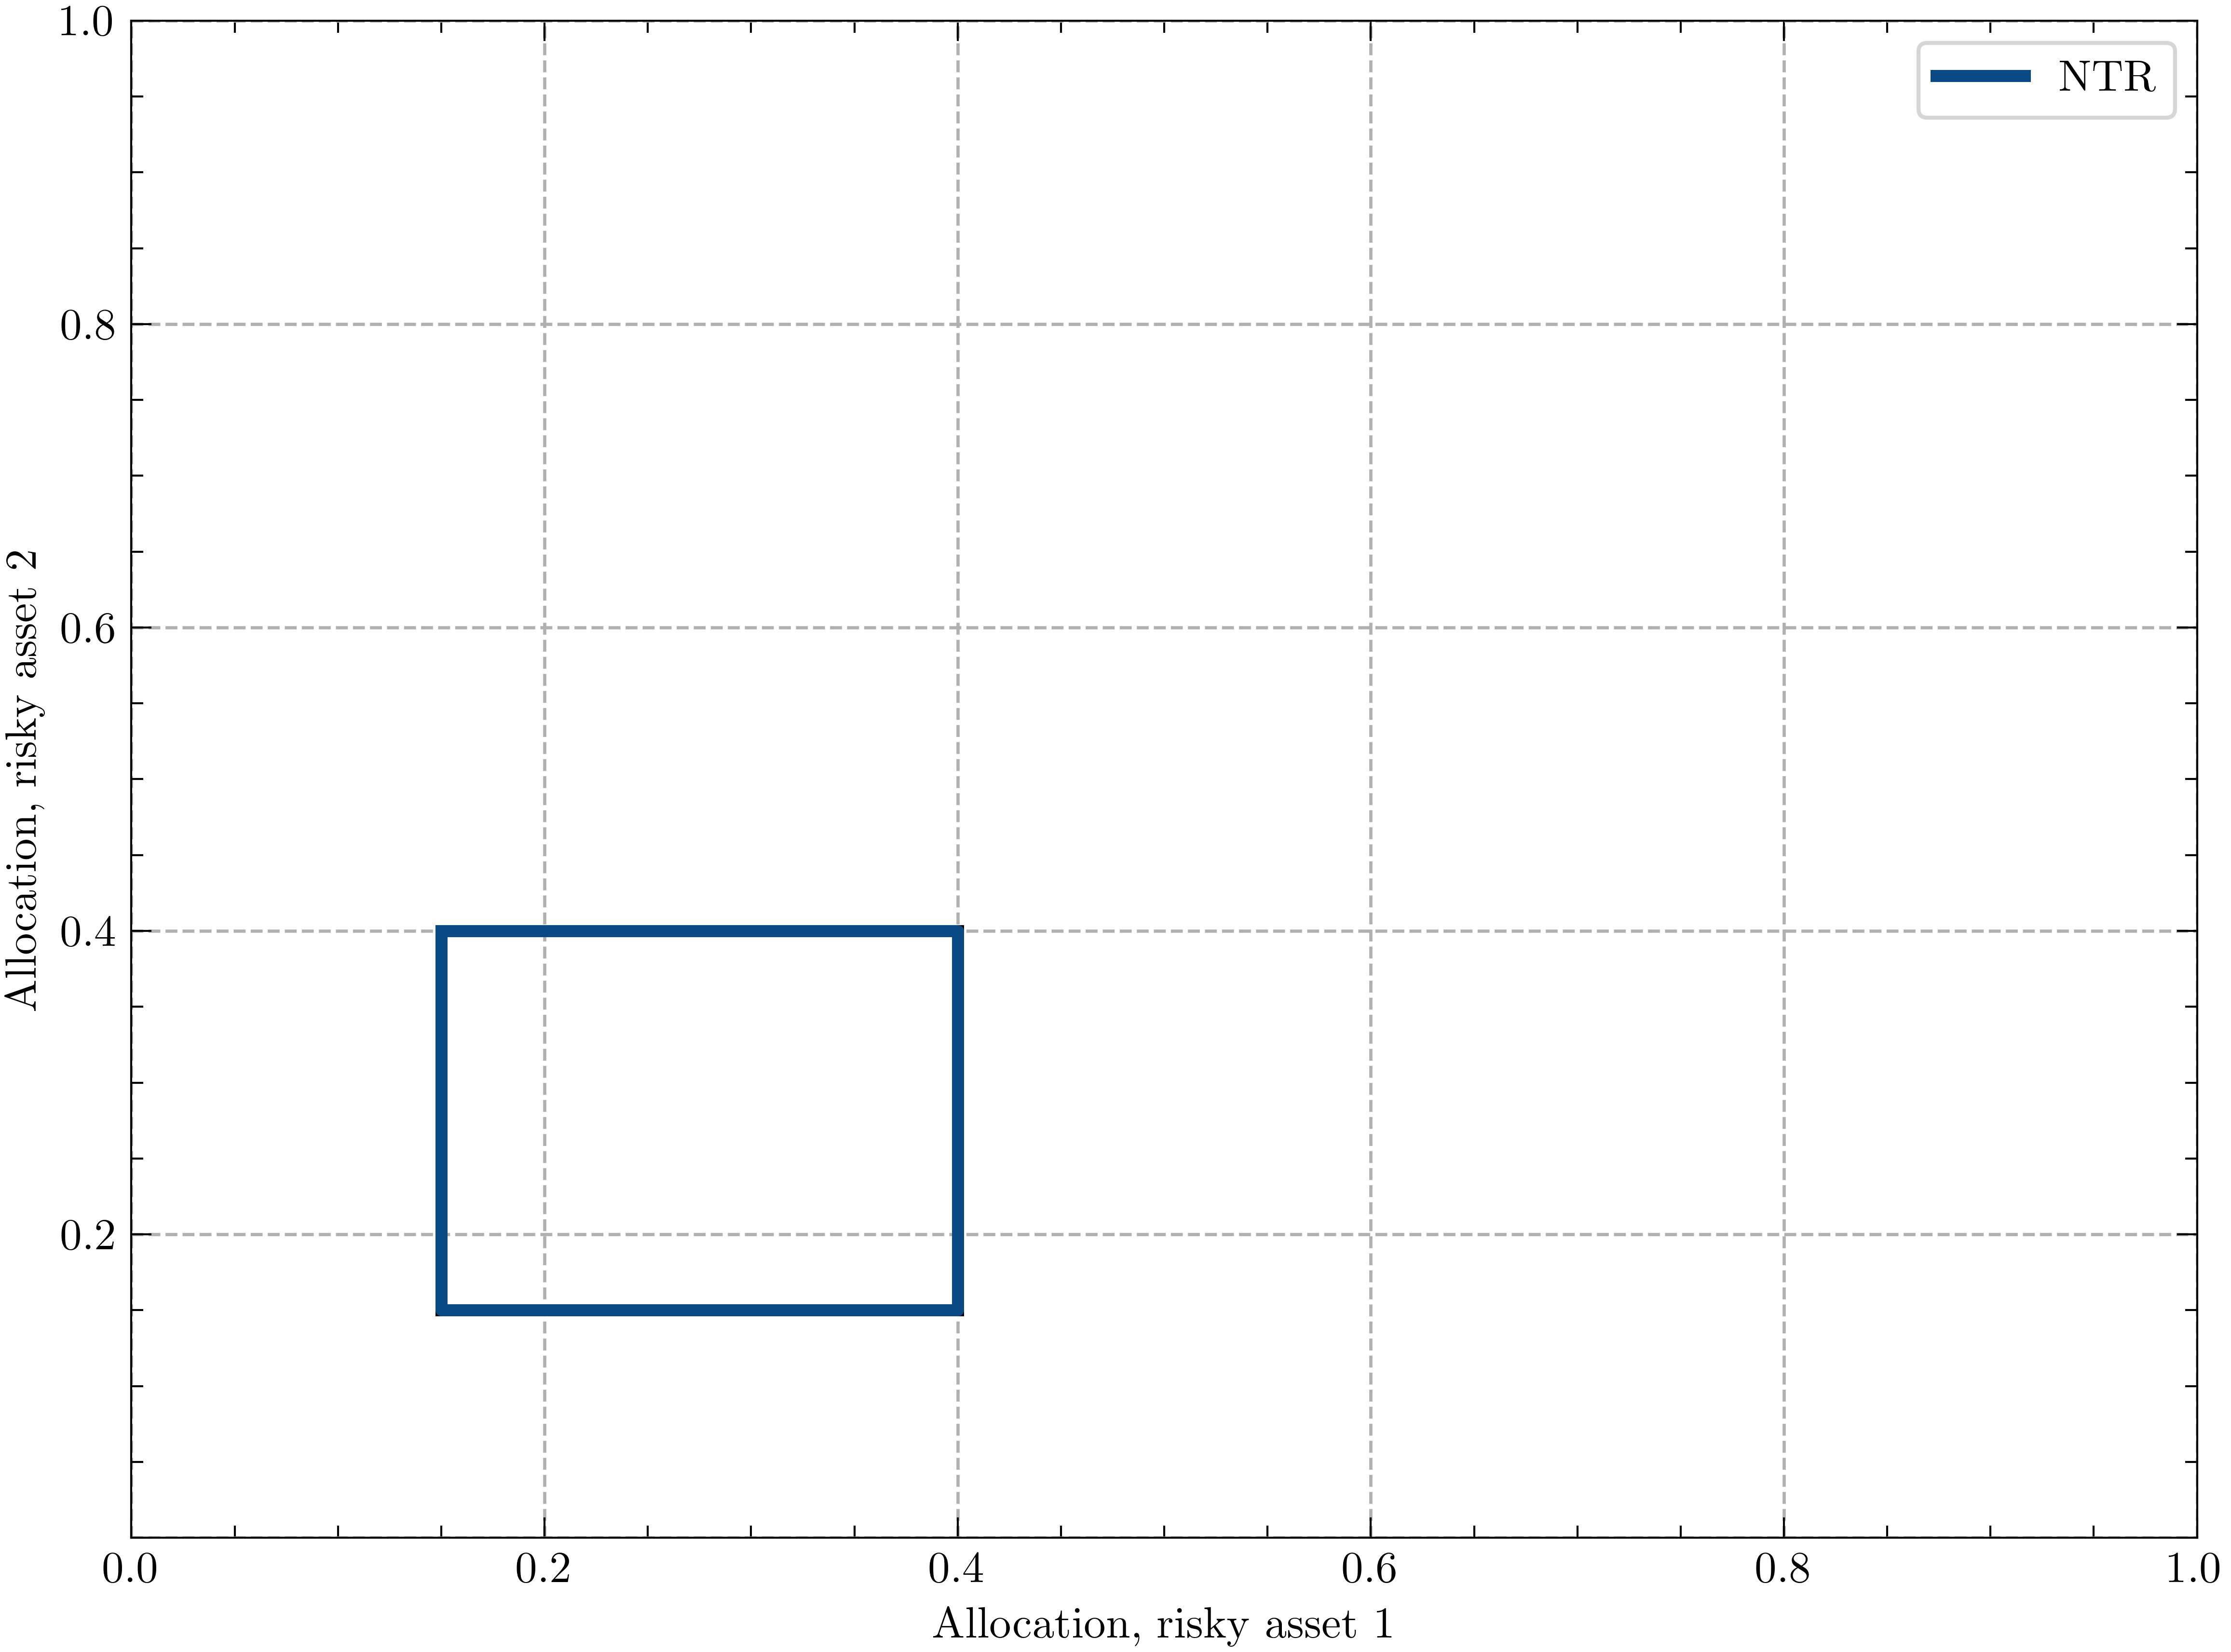
\includegraphics[scale=0.38]{Example_NTR.png}
  \end{center}
  % \floatfoot{\textbf{Note:}}
\end{figure}
The square shape of the \ac{NTR} occurs with proportional transaction costs
and independent (i.i.d) risky assets. However the NTR is not always a perfect square, for more on this see \autocite{Dybvig2020}.


\subsection{Base problem: Portfolio choice with proportional costs and consumption}\label{Subsection: Base_Problem}
Considering the class of problems constructed in the prior section,
we can now quickly introduce the basic problem formulation.
We consider an investor with CRRA utility function. She can invest in one risk free asset and $k$ risky assets.
Trading is subject to proportional transaction costs hence we have the following cost function (in cumulative terms):
\begin{equation} \label{eq: base_model_transaction-cost}
  \psi (\boldsymbol{\delta}^{+}_{i,t}, \boldsymbol{\delta}^{-}_{i,t} ) = \tau (\boldsymbol{\delta}^{+}_{i,t} + \boldsymbol{\delta}^{-}_{i,t}) 
\end{equation}
We do not assume that returns are dependent on stochastic parameters, but instead are drawn from a distribution with known parameters.
Hence we assume \( \theta_{t} = \theta \) for all $t$. That is that we assume a constant return on the risk free asset, hence $R_{f}(\theta_t) = R_{f}$,
and the risky assets follow a multivariate log-normal distribution, with some mean and covariance matrix.
We can now formulate the entire problem giventhe class structure from section \ref{Subsection: Dynamic-portfolio-choice}.
The terminal value function is given by equation \eqref{eq: class_terminal_value}. 
The system is subject to the constraints of equations \eqref{eq: No_Short_risky}, \eqref{eq: No_Short_bonds} and \eqref{eq: No_Geared_Risky},
as well as a simple constrain on consumption, $c_t \geq 0$.
We assume that the position in bond holdings is the residual wealth, and they therefore follow the process
in \eqref{eq: class_bond_holdings}. The Bellman equation is therefore:
\[  
  v_{t} (\mathbf{x}_{t}, \theta_t) = \max_{c_t , \boldsymbol{\delta}^{+}_{t}, \boldsymbol{\delta}^{-}_{t}  },  \{ u(c_t) 
  \Delta t + \beta \mathbb{E}_{t} \left[ 
    \pi_{t+\Delta t}^{1-\gamma}
    v_{t+\Delta t} (\mathbf{x}_{t+\Delta t }) 
    \right] \} , \quad t < T 
\]
With same terminal condition as before, where investments are sold and wealth is consumed.
\[
  v_T (\mathbf{x}_T) = u  (1 - \psi( \mathbf{0},\mathbf{x}_T))
\]

\subsection{Portfolio choice with fixed costs}
I now consider the model, where the investor faces fixed costs when rebalancing the portfolio, instead of proportional costs.
Fixed costs are common in practice, and can be seen as a fixed fee for trading, regardless of the traded amount.
I consider a slight modification to the classical purely fixed costs, and instead consider fixed costs as a percentage of the wealth.
I do this to be able to use the same model structure as in section \ref{Subsection: Base_Problem}, where variables are in fractions of wealth,
in order to drop wealth as a state variable.\\
This is seen previously in \autocite{morton1995optimal}, who note that such a fixed cost can be seen as a portfolio management fee.
In practice, when setting the level of the fixed cost, i make an implicit assumption on the wealth of the investor,
if i want to draw comparisons to common trading fees on the market, as the fixed cost in this scenario is purely fixed.
The cost function is then given by:
\begin{equation}
  \label{eq:Fixed_Cost_Function}
  \psi (\boldsymbol{\delta}^{+}_{t}, \boldsymbol{\delta}^{-}_{t} ) = \mathbf{1} \left(  \sum^{k}_{i=1} \delta^{+}_{i,t} + \delta^{-}_{i,t}  > 0 \right) \cdot \operatorname{fc}
\end{equation}
Where $\operatorname{fc}$ is the fixed cost, and $\mathbf{1}(\cdot)$ is the indicator function.
The fixed cost is only incurred if the investor rebalances the portfolio, and is independent of the traded amount.
The normaized bond holdings are therefore given by:
\begin{equation}\label{eq: fx_bond_holdings}
  b_{t} = 1 - \mathbf{1}^{\top} \cdot (\mathbf{x_t} - \boldsymbol{\delta}_t -) - \psi( \boldsymbol{\delta}^{+}_{t}, \boldsymbol{\delta}^{-}_{t} ) - c_t \Delta t
\end{equation}
The model otherwise remains the same as in section \ref{Subsection: Base_Problem}, with the same constraints and dynamics, while using the new cost function.
Note that in the terminal period, when all investments are sold, the fixed cost is incurred, unless the investor holds no risky assets.
Note that for the model to be well defined, the fixed cost must be less than the wealth of the investor, as the fixed cost is a percentage of the wealth.
Furthermore, the fixed cost function is not differentiable. Furthermore \autocite{Dybvig2020} notes that the fixed cost only problem,
is not a convex optimization problem, and is therefore not as easily solved as the proportional cost problem. I will deal with these issues individually
when implementing the model.
\subsection{Portfolio choice with fixed and proportional costs}
The last model i consider is a combination of the two previous models, where the investor faces both fixed and proportional costs.
This is a more realistic model, as it combines the two most common types of transaction costs an individual common investor 
face in the real world, with a fixed brokerage fee and a percentage of the traded amount stemming from bid ask spreads, taxes or commisions \autocite{Lesmond1999}.
The cost function is then given by:
\begin{equation}
  \label{eq:Fixed_Proportional_Cost_Function}
  \psi (\boldsymbol{\delta}^{+}_{t}, \boldsymbol{\delta}^{-}_{t} ) = \mathbf{1} \left(  \sum^{k}_{i=1} \delta^{+}_{i,t} + \delta^{-}_{i,t}  > 0 \right) \cdot \operatorname{fc} + \tau (\boldsymbol{\delta}^{+}_{t} + \boldsymbol{\delta}^{-}_{t})
\end{equation}
The normalized bond holdings are therefore given by:
\begin{equation}\label{eq: fx_bond_holdings}
  b_{t} = 1 - \mathbf{1}^{\top} \cdot (\mathbf{x_t} - \boldsymbol{\delta}_t -) - \psi( \boldsymbol{\delta}^{+}_{t}, \boldsymbol{\delta}^{-}_{t} ) - c_t \Delta t
\end{equation}
The model otherwise remains the same as in section \ref{Subsection: Base_Problem}, with the same constraints and dynamics, while using the new cost function.

\ifdefined\COMPILINGMAIN
% Main file is compiling this section, skip the end
\else
\printbibliography
\end{document}
\fi